\documentclass[AtomicOptical1Notes.tex]{subfiles}

\begin{document}

\begin{center}\huge Week 2: Quantized Spin in a Magnetic Field\end{center}

\section{Equation of motion for the expectation value}

	\subsection{Quantized spin in a magnetic field}
		\begin{itemize}
			\item Everything we have learned about classical magnetic moment exactly applies to quantum version.
			\item Hamiltonian for an atom in a magnetic field: $ H=-\v{\mu}\v{B_0}=-\gamma\v{L_z}B_0 $.
			\item Heisenberg equation of motion for any operator: $ \d{\hat{O}}{t}=\frac{i}{\hbar}[\hat{H},\hat{O}] $.
			\item Using the above equation and the hamiltonian we get simple equation of motion for the system: $ \d{\hat{\mu}}{t}=\gamma\hat{\mu}\times\v{B} $. It looks exactly as a classical result and is valid for any value of spin.
			\item Any two-level system can be regarded as spin $\frac{1}{2}$ system and it just precesses (unless magnetic field is very strong).
			\item Valid for a system of N two-level systems $\Rightarrow$ Dicke superradiance.

Superradiance is a phenomenon of collective emission of an ensemble of excited atoms or ions, first considered by Dicke. It is similar to superfluorescence, but it starts with the coherent excitation of the ensemble, usually with an optical pulse. This coherence (i.e. a well-defined phase relationship between the excitation amplitudes of lower and upper electronic states) leads to a macroscopic dipole moment. The maximum intensity of the emitted light scales with the square of the number of atoms, because each atom contributes a certain amount to the emission amplitude, and the intensity is proportional to the square of the amplitude. As the number of photons rises in a kind of chain reaction, Dicke later (in a patent application) described the phenomenon of superradiance as an optical bomb. \href{https://www.clear.rice.edu/elec603/spring2008/Selecting_a_Paper_files/Physical%20Review%201954%20Dicke.pdf}{\color{blue} \underline{Link to the Dicke's paper.}}
		\end{itemize}
		
\section{The two-level system: spin $\frac{1}{2}$}

	\subsection{Two-level system - spin $\frac{1}{2}$ Rabi oscillations}
		\begin{itemize}
			\item An electron in a magnetic field is in its ground state while being anti-aligned with the field (it has lower energy than when being aligned) because the electron has negative gyromagnetic ratio.
			\item Probability to find the system in the excited state at time t if it was in ground state at time $t=0$ (Rabi transition probability): $ P= \frac{\omega_R^2}{\Omega_R^2} \sin^2 \frac{\Omega_R t}{2} $.
			
			\begin{center}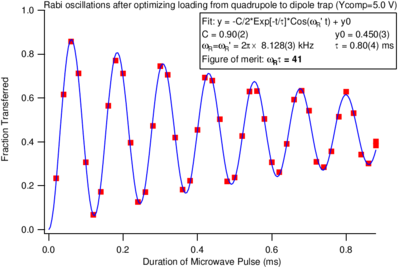
\includegraphics[scale=0.75]{rabiresonance}\end{center}
			
		\end{itemize}

\subsection{Two-level system Hamiltonian}
		\begin{itemize}
			\item The famous 'dressed atom' Hamiltionian in the so called 'rotating wave approximation':
			
			\begin{center} $ \hat{H} = \frac{\hbar}{2} \left( \begin{array}{cc}
										   \omega_0 & \omega_Re^{-i\omega t} \\
										   \omega_Re^{i\omega t} & -\omega_0 \end{array}
											 \right) $ \end{center}
	
That expression is exact. Its eigenstates and eigenvalues provide a very elegant, very intuitive solution to the two-state problem. It describes two-level system + one mode of the e-m field with arbitrary amplitude.
			\item The Hamiltonian can be easily solved after the unitary transformation: $ R = \left( \begin{array}{cc}
									e^{\frac{i\omega t}{2}} & 0 \\
									0 & e^{-\frac{i\omega t}{2}} \end{array}
									\right) $ which is a rotation operator and it makes the problem time independent. After the transformation we get a Hamiltonian: $ \hat{H}'=\frac{\hbar}{2} \left( \begin{array}{cc}
								 \delta & \omega_R \\
								 \omega_R & \delta \end{array}
								 \right)$ (where $ \delta = \omega_0-\omega $ is a detuning) that can be easily solved and we get the same answer as before (Rabi transition probability).
			
		\end{itemize}

\section{Rapid adiabatic passage - quantum treatment}

	\subsection{Rapid adiabatic passage and Landau-Zener transitions}
		\begin{itemize}
			\item We can use previous results to make a graph. The dashed line comes from the basic Hamiltonian and the curves are caused by the driving Hamiltonian. 
			
			\begin{center}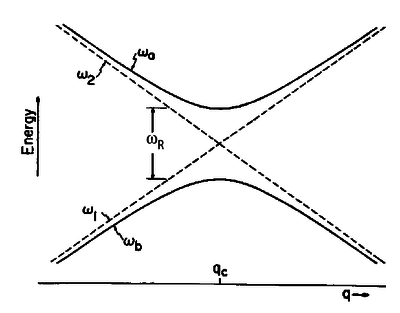
\includegraphics[scale=0.75]{landauzener}\end{center}
			
			\item When we sweep the frequency $\omega$ at a rate $\dot\omega$ through the resonance (change $\delta$) we realize Landau-Zener problem of a sweep through the avoided crossing which is a quantum mechanical description of rapid adiabatic passage. Probability of a jump at the crossing that happens when the sweep is sufficiently rapid is: $ P=e^{-2\pi\Gamma} $ where $ \Gamma = \frac{1}{4}\frac{\omega_R^2}{\dot\omega} $ is the Landau-Zener parameter. Adiabaticity requires that $ \frac{\omega_R^2}{\dot\omega}\gg 1 $. The process is coherent.
			
		\end{itemize}

\end{document}